\newpage
\hypertarget{multiMOSL}{}
\subsection{Working with multple MOSL projects}
\texHeader

\begin{itemize}

\item[$\blacktriangleright$] Press the \texttt{new} button on the Eclipse toolbar and navigate to ``Examples/eMoflon Handbook Examples/''
(Fig.~\ref{eclipse:dictionaryDownloadWizard}). Find and select \texttt{Visual Dictionary Language} to copy a new \texttt{Dictionary} metamodel project into your
workspace.

\begin{figure}[htbp]
\begin{center}
  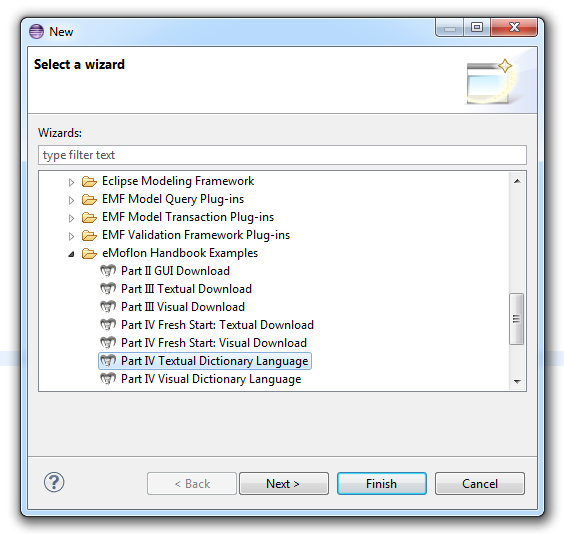
\includegraphics[width=0.8\textwidth]{eclipse_part4DictionaryLanguageDownload}
  \caption{Download the textual Dictionary project}
  \label{eclipse:dictionaryDownloadWizard}
\end{center}
\end{figure}

\item[$\blacktriangleright$] If successful, your workspace should resemble Fig.~\ref{eclipse:loadedDictionaryMetamodel}. It would be a good idea to inspect the
metamodel until you feel comfortable with what you'll be working with. This transformation will be focusing on transformation on the \texttt{Dictionary} and
\texttt{Entry} eclasses.

\item[$\blacktriangleright$] While you now have your source and target metamodels in the same place, \texttt{LeitnersLearningBox} still needs to be told to
access \texttt{DictionaryLanguage}. navigate to ``LeitnersLearningBox/MOSL/MyWorkingSet'' and open \texttt{\_imports.mconf}
(Fig.~\ref{eclipse:importConfigFile}) and add the statement: 
\syntax{import Dictionary}

\newpage

\begin{figure}[htbp]
\begin{center}
  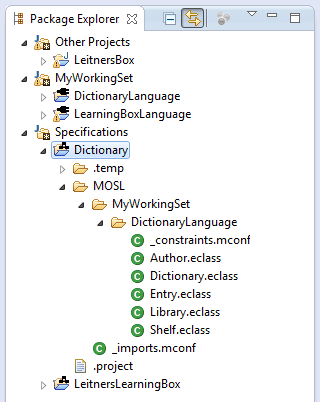
\includegraphics[width=0.5\textwidth]{eclipse_loadDictionaryMetamodel}
  \caption{\texttt{DictionaryLanguage}'s metamodel structure}
  \label{eclipse:loadedDictionaryMetamodel}
\end{center}
\end{figure}

\vspace{1cm}

\begin{figure}[htbp]
\begin{center}
  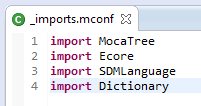
\includegraphics[width=0.35\textwidth]{eclipse_learningBoxImportFile}
  \caption{Importing \texttt{Dictionary} into the learning box}
  \label{eclipse:importConfigFile}
\end{center}
\end{figure}

\vspace{1cm}

\item[$\blacktriangleright$] Save and rebuild \texttt{LeitnersLearningBox}. You're ready to start a TGG transformation as soon as it completes! It should be
mentioned that you could have achieved the equivalent result by copying the \texttt{DictionaryLanguage} folder into \texttt{LeitnersLearningBox}'s working set.

\end{itemize}
